%=================
%     PACKAGES
%=================
\usepackage{graphicx,latexsym}
\usepackage{amssymb,amsthm,amsmath}
\usepackage{physics}
\usepackage{longtable,booktabs,setspace}
\usepackage[hyphens]{url}
\usepackage{rotating}
\usepackage{natbib}
\usepackage{dsfont} % Boldface 1 for indicator function
\usepackage{array} % For the analytical eigenvector proof (block matrices)
% \usepackage{times} % other fonts are available like times, bookman, charter, palatino

% For code snippet environments
\usepackage{listings}
\usepackage[svgnames]{xcolor}

% For stitching the code appendix
\usepackage{pdfpages}
%\usepackage{markdown} % For using `script.R` md in code appendix
%\usepackage[hashEnumerators,smartEllipses]{markdown}

%=====================
%     ENVIRONMENTS
%=====================
% Theorems
\newtheorem{theorem}{Theorem}[section]
\setlength{\parskip}{0pt}
\setlength\parindent{24pt}

% Defintions
\newtheorem{definition}{Definition}[section]
\setlength{\parskip}{0pt}
\setlength\parindent{24pt}

% Examples
\newtheorem*{example}{Example}
%\newtheorem{example}{Example}[section]
\setlength{\parskip}{0pt}
\setlength\parindent{24pt}

% Code Examples
\newtheorem*{code}{Code Example}
%\newtheorem{code}{Code Example}[section]
\setlength{\parskip}{0pt}
\setlength\parindent{24pt}

% Notes
\newtheorem*{note}{Note}
%\newtheorem{note}{Note}[section]
\setlength{\parskip}{0pt}
\setlength\parindent{24pt}

% Algorithms
\newtheorem{algorithm}{Algorithm}[section]
\setlength{\parskip}{0pt}
\setlength\parindent{24pt}
%\newtheorem*{algorithm}{Algorithm}%[section]

% Remarks
\newtheorem*{remark}{Remark}
%\newtheorem{remark}{Remark}[section]
\setlength{\parskip}{0pt}
\setlength\parindent{24pt}

% R Code Chunks
%code snippet environments V1

\lstset{language=R,
    basicstyle=\small\ttfamily,
    stringstyle=\color{DarkGreen},
    otherkeywords={0,1,2,3,4,5,6,7,8,9},
    morekeywords={TRUE,FALSE},
    deletekeywords={data,frame,length,as,character},
    keywordstyle=\color{blue},
    commentstyle=\color{DarkGreen},
}

\xdefinecolor{gray}{rgb}{0.4,0.4,0.4}
\xdefinecolor{blue}{RGB}{58,95,205}% R's royalblue3; #3A5FCD

% Mini title document environment
\newcommand{\minititle}[1]{
  \begin{center}
    \textbf{#1}
  \end{center}
}
%==================
%     COMMANDS
%==================
% Latin Letters (bb)
\newcommand{\Cc}{\mathbb{C}} % Complex Numbers
\newcommand{\R}{\mathbb{R}} % Reals
\newcommand{\N}{\mathbb{N}} % Naturals
\newcommand{\F}{\mathbb{F}} % Field

% Latin Letters (cal)
\newcommand{\B}{\mathcal{B}} % Batch
\newcommand{\Rseq}{\mathcal{R}} % Ratio-Sequence
\newcommand{\Seq}{\mathcal{S}} % Sequence
\renewcommand{\S}{\mathbb{S}} % Spectrum
\newcommand{\Ens}{\mathcal{E}} % Ensemble
\newcommand{\D}{\mathcal{D}} % Distribution

% Greek letters
\renewcommand{\epsilon}{\varepsilon}
\newcommand{\ep}{\epsilon}
\renewcommand{\d}{\delta}
\renewcommand{\b}{\beta}

% Probability & Probability Distributions
\newcommand{\Prb}{\text{P}}
\newcommand{\E}{\mathbb{E}}
\newcommand{\Var}{\text{Var}}
\newcommand{\Unif}{\text{Unif}}
\newcommand{\Bern}{\text{Bern}}
\newcommand{\Bin}{\text{Bin}}
\newcommand{\Normal}{\mathcal{N}}

% Math macros
\newcommand{\oneto}[1][n]{1,\dots,#1} % 1,...,n
\newcommand{\sumi}[1][n]{\sum_{i = 1}^{#1}} % sum from i = 1 to n
\newcommand{\seq}[2][n]{{{#2}_0,{#2}_1,\dots,{#2}_{#1}}} % x_1,...,x_n

% Words
\newcommand{\where}{\text{ where }}
\newcommand{\for}{\text{ for }}
\newcommand{\given}{\text{ given }}
\renewcommand{\and}{\text{ and }}

% Other
\newcommand{\ra}{\rightarrow}

%==================
%     TABLES
%==================
%============================
%      D-DISTRIBUTIONS
%============================
\newcommand{\Ddisttable}{
  \begin{tabular}{ |p{3cm}||p{3cm}|p{3cm}|p{3cm}|  }
   \hline
   \multicolumn{4}{|c|}{Table of Random Matrix Distributions} \\
   \hline
   Distribution & Notation ($\D$) & Parameters & Class\\
   \hline
   Normal & $\Normal(\mu,\sigma)$ & $\mu \in \R, \sigma \in \R^+$  &  Explicit\\
   Uniform  & $\Unif(a,b)$ & $a,b \in \R$ & Explicit\\
   Hermite-$\beta$   & $\mathcal{H}(\beta)$  &  $\b \in \N$  & Implicit\\
   Erdos-$p$   &   $\text{ER}(p)$  & $p \in [0,1]$   & Implicit\\
   \hline
  \end{tabular}
}
%============================
%      SPECTRUM SCHEMES
%============================
\newcommand{\spectrumschemetable}{
  \begin{tabular}{ |p{3cm}||p{2cm}|p{2.5cm}|p{4.5cm}|  }
   \hline
   \multicolumn{4}{|c|}{Table of Spectrum Schema} \\
   \hline
   Scheme & Matrix & Notation & Ordering \\
   \hline
   Sign-Ordered & $P$ & $\sigma_{S}(P)$ & $\lambda_1 \geq \lambda_2 \geq ... \geq \lambda_N$ \\
   Norm-Ordered & $P$ & $\sigma_{N}(P)$ & $|\lambda_1| \geq |\lambda_2| \geq ... \geq |\lambda_N|$ \\
   Singular & $P \cdot P^T$ & $\sigma_{+}(P)$ & $\sqrt{\lambda_1} \geq \sqrt{\lambda_2} \geq ... \geq \sqrt{\lambda_N}$ \\
   \hline
  \end{tabular}
}
%============================
%     DISPERSION METRICS
%============================
\newcommand{\dispersiontable}{
  %\begin{tabular}{ |p{5cm}||p{2cm}|p{2cm}|p{2cm}|p{2cm}|  }
  \begin{tabular}{ |p{4.4cm}||p{1.9cm}|p{1.9cm}|p{1.9cm}|p{1.9cm}|  }
   \hline
   \multicolumn{5}{|c|}{Table of Dispersion Metrics} \\
   \hline
   Metric* & Notation & Formula & Symmetric & Parameters\\
   \hline
   Standard Norm & $\d$ & $|z' - z|$ &  True & - \\
   $\beta$-Norm & $\d_\b$ & $|z' - z|^\b$ & True & $\b \in \N$ \\
   Difference of Absolutes & $\d_{\text{abs}}$ & $|z'| - |z|$ &  False  &  - \\
   Identity Difference &  $\d_{\text{id}}$ & $z' - z$ & False &  - \\
   %Angola & AO & AGO & 024\\
   \hline
  \end{tabular}
}
%============================
%      PAIRING SCHEMES
%============================
\newcommand{\pairingschemetable}{
  %\begin{tabular}{ |p{2.5cm}||p{1.75cm}|p{5.5cm}|  }
  %\begin{center}
    \begin{tabular}{ |p{3cm}||p{3cm}|p{6cm}|  }
     \hline
     \multicolumn{3}{|c|}{Table of Pairing Schema} \\
     \hline
     Scheme & Notation & Formula \\
     \hline
     Lower & $\Pi_<$ & $\{(i,j) \mid i < j \for i,j \in \N_N \}$ \\
     Upper  & $\Pi_>$ & $\{(i,j) \mid i > j \for i,j \in \N_N \}$ \\
     Consecutive  & $\Pi_C$ & $\{(i,j) \mid i = j + 1 \for i,j \in \N_N \}$ \\
     All & $\Pi_0$ & $\{(i,j) \mid i,j \in \N_N \}$ \\
     \hline
    \end{tabular}
  %\end{center}
}


%==================
%     GRAPHICS
%==================
%==================
%     CHAPTER 2
%==================

\newcommand{\FIGUREspectrumcomparison}[2]{
  \begin{figure}[#1]
   \begin{center}
    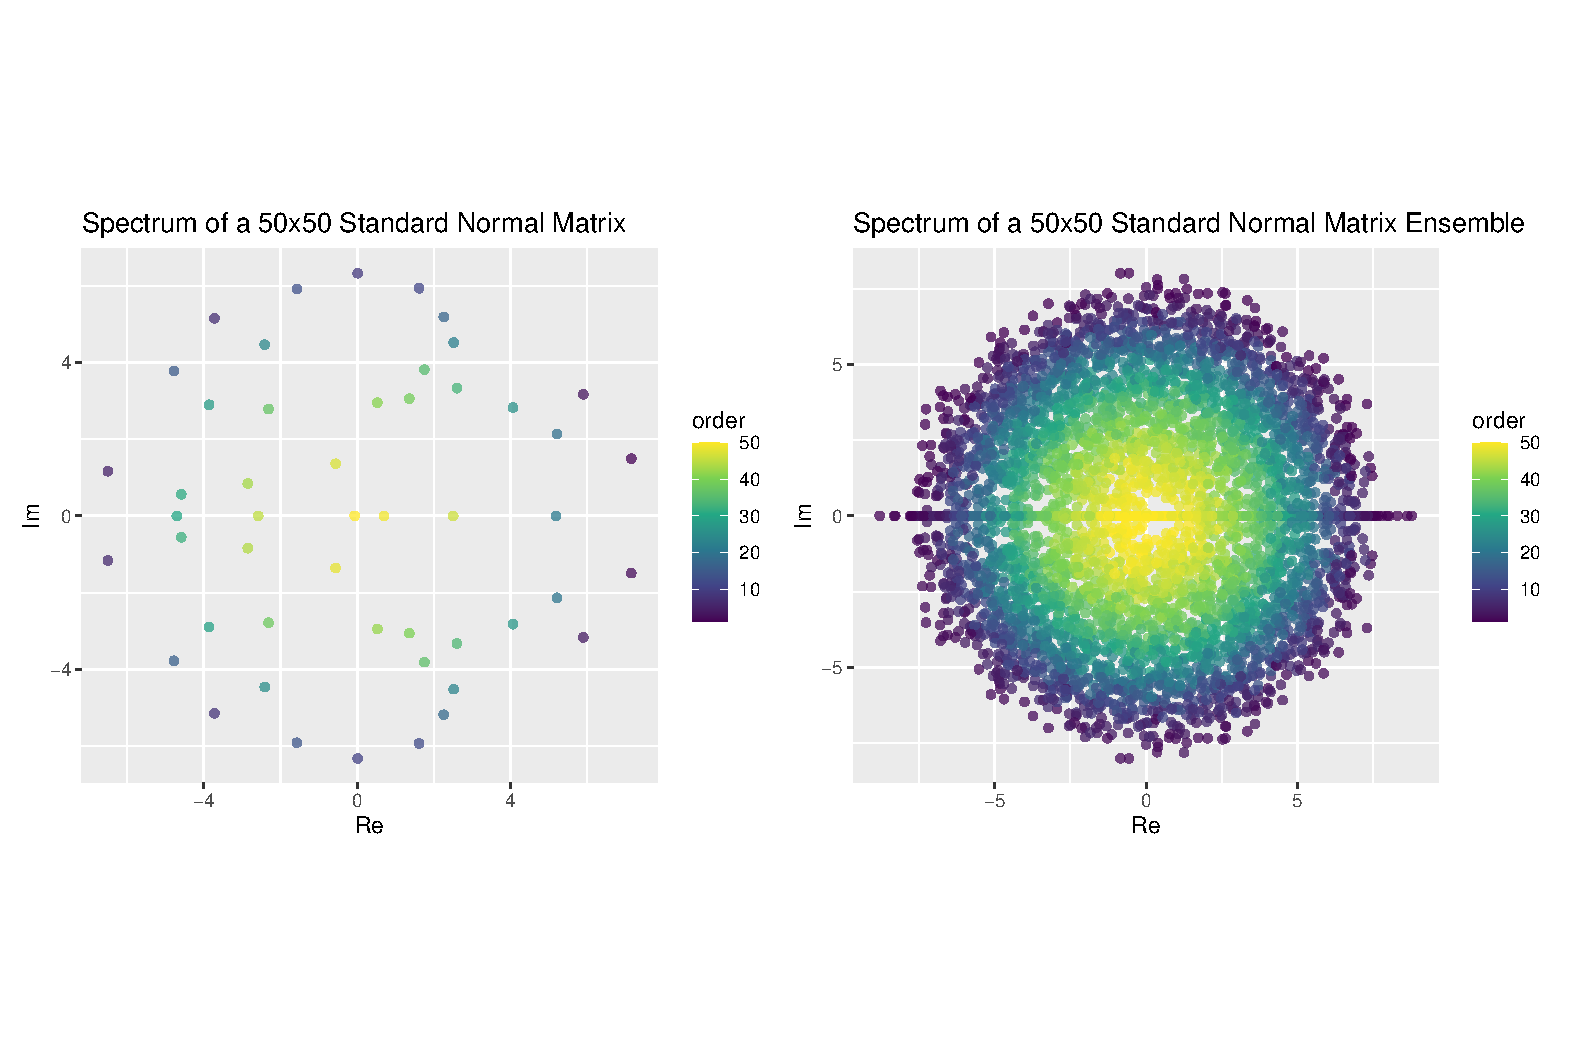
\includegraphics[scale = #2]{../graphics/chap2/2-1-2_comparison}
    \caption{Spectrum of a Matrix versus an Ensemble}
   \end{center}
   \label{ensemble_comparison_plot}
  \end{figure}
}

\newcommand{\FIGUREnormalspectrum}[2]{
  \begin{figure}[#1]
   \begin{center}
    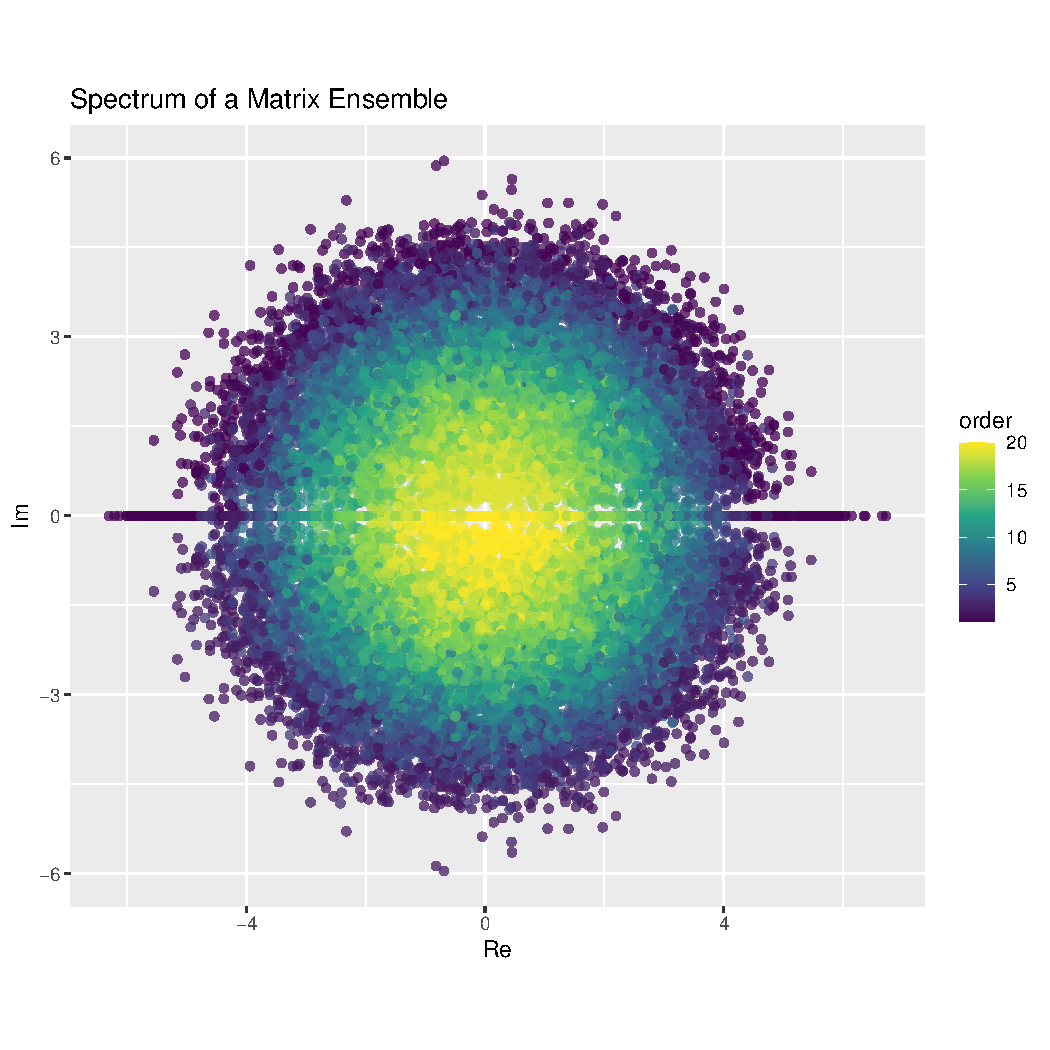
\includegraphics[scale = #2]{../graphics/chap2/2-1-2_normal_spec}
    \caption{Spectrum of a Standard Normal Matrix ensemble}
   \end{center}
   \label{spectrum_normal_ensemble_plot}
  \end{figure}
}

\newcommand{\FIGUREorderscheme}[2]{
  \begin{figure}[#1]
   \begin{center}
    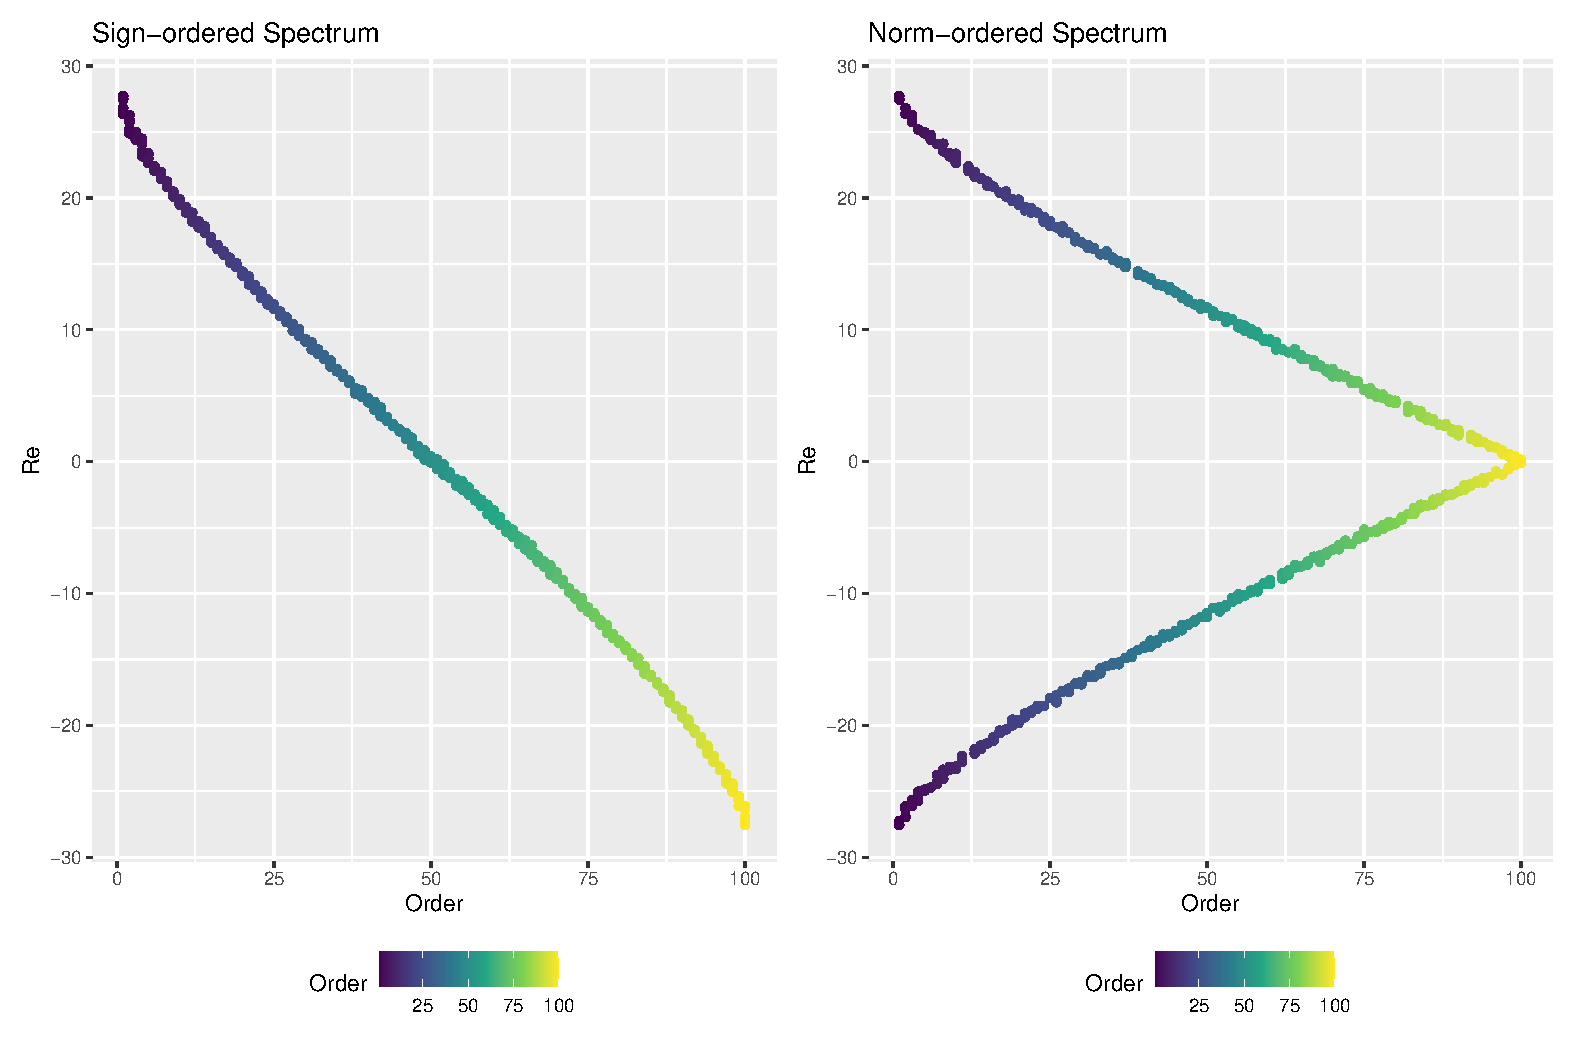
\includegraphics[scale = #2]{../graphics/chap2/2-2-1_orderscheme}
    \caption{Spectrum displaying two different ordering scheme}
   \end{center}
   \label{orderscheme_plot}
  \end{figure}
}

\newcommand{\FIGUREsemicircle}[2]{
  \begin{figure}[#1]
   \begin{center}
    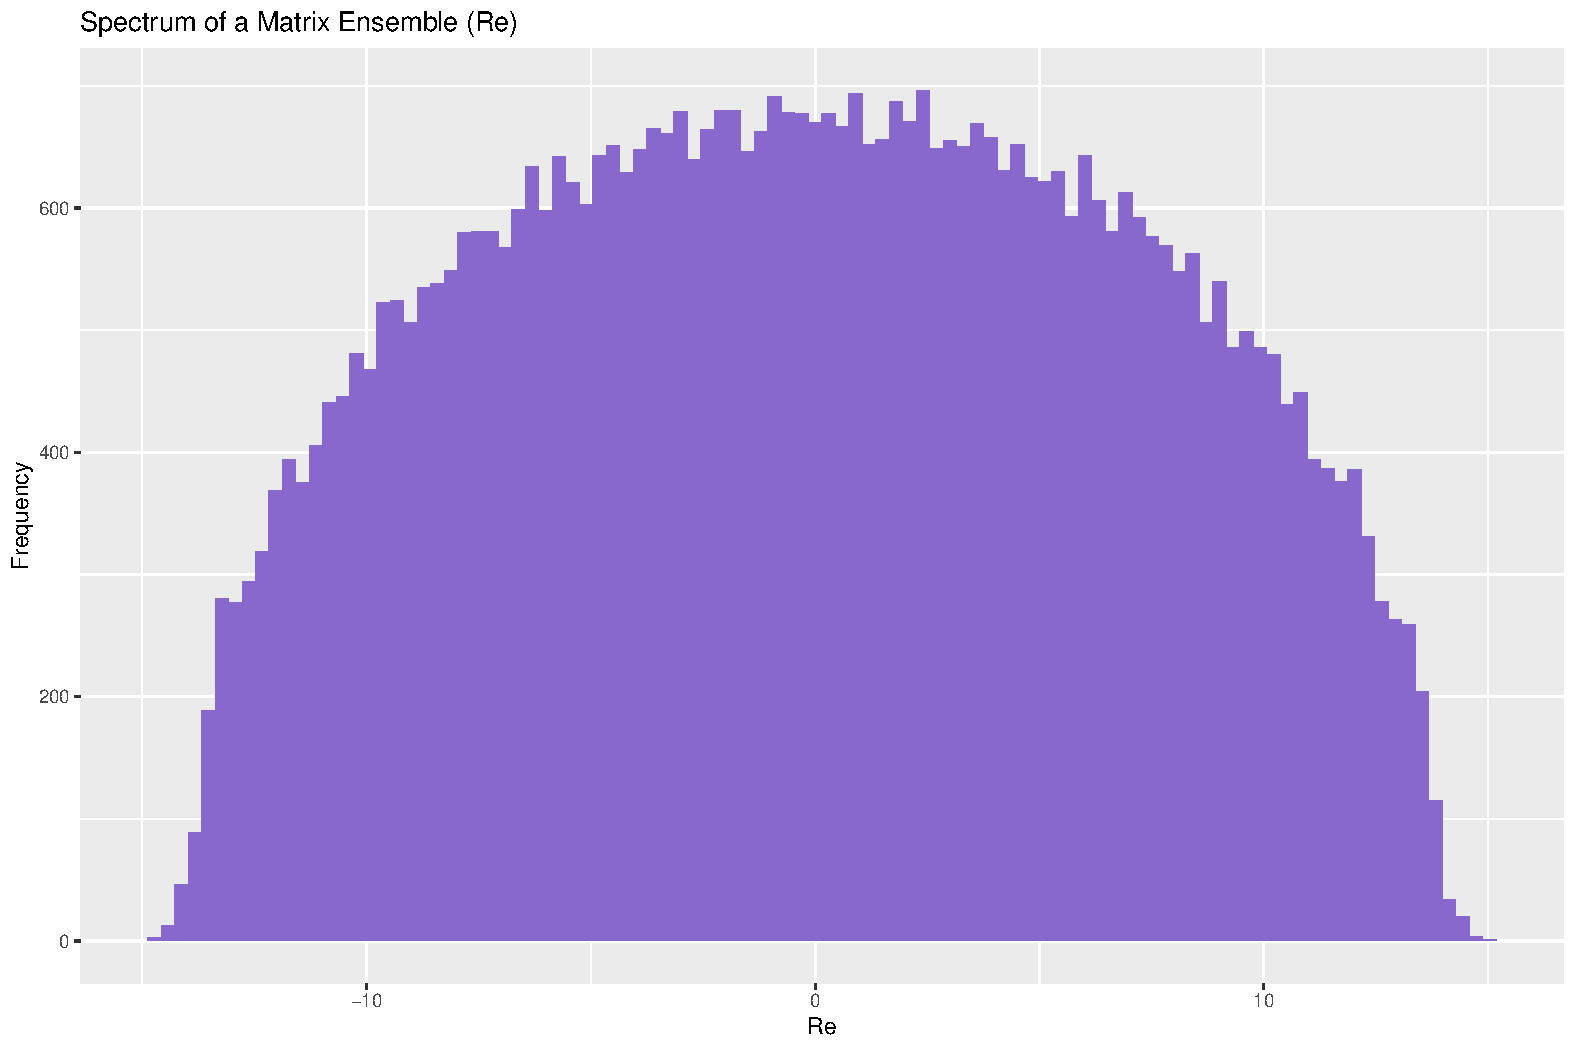
\includegraphics[scale = #2]{../graphics/chap2/2-3-2_semicircle}
    \caption{Eigenvalues of a Symmetric Matrix displaying the Semicircle Distribution}
   \end{center}
   \label{semicircleplot}
  \end{figure}
}
%==================
%     CHAPTER 3
%==================

%==================
%     CHAPTER 4
%==================s

